\section{itération 1 : nouveau BS au standard MQTT}
    \subsection{Conception de la première itération}
        \gls{mdi}, étant une entreprise innovante en télématique, doit toujours
        suivre et avancer les nouvelles technologies. Une de ces technologies
        est le protocol de communication standar des objets connectés: le MQTT.

        ...
        Le protocole- Vehicle to Everything - donne au véhicule la
        connaissance de son environement en collectant les informations des autres
        utilisateurs de ce protocole, et contribue aux connaissances collectives en
        diffusant les siennes.\\[0.3cm]
        Actuellement, \gls{mdi} utilise une stack \gls{v2x} developpée par Marben\cite{marben_site}.
        Cette stack, écrite en C++, ne répond pas aux demandes de performance de
        l'entreprise, et introduit une dépense évitable en coûts de license.\\[0.3cm]
        Le but de ce projet est de développer une stack \gls{v2x} pour remplacer celle
        de Marben, et qui procure les performances nécessaires pour tourner sur les
        boitiers. Ce sujet ne sera pas trop détaillé vu qu'il a été abandonné par l'entreprise.


    \subsection{Descriptif du protocole:Le standard MQTT, l'essentiel à savoir}
        Voir les couches de MQTT
        Ce protocole s'intéresse à toutes les couches de communication du modèle OSI.
        Les spécifications exactes diffèrent entre l'Union Européenne, les Etats Unis,
        et le Japon.

        \subsubsection{La couche physique}
           v2x définit un protocole dérivé du wifi: le 802.11p, nommé \gls{wave}.
            Ce protocole plus lent, mais plus adapté sert aux communications entre
            véhicules à haute vitesse, et entre ces véhicules et des stations intelligentes.
            Les connexions 3G et 4G ont l'inconvenient d'une grande latence, et sont donc
            éliminées comme vecteurs pour le protocole. En effet, \gls{v2x} a besoin
            d'établir des connexions directes entre véhicules, pour assurer une latence
            petite, et bornée.
            Une communication par 5G, la C-V2X (Cellular V2X), est envisagée vers
            2025: les specs du 5G répondent aux demandes de latence pour \gls{v2x}.
            Aujourd'hui, \gls{mdi} utilise le module Vera-P174\cite{vera_doc}
            pour cette couche.


        \subsubsection{La couche transport}
            \gls{v2x} utilise les protocols TCP et UDP sur IPv6. Il utilise en plus
            le protocol \gls{wsmp}\cite{wave_spec}. Dans un premier temps, \gls{mdi}
            s'intéresse à un modèle sans \gls{wsmp}. Actuellement, la couche transport
            est implémentée par la stack Marben.

        \subsubsection{La couche applicative}
            La couche applicative de ce protocole consiste en un nombre d'applications
            essentielles et non essentielles. Les différentes stations \gls{v2x}, ou
            station \gls{its}, communiquent, en broadcast, plusieurs types de messages,
            dont les plus importants sont les \gls{cam}s et les \gls{denm}s.\\[0.3cm]
            Les \gls{cam}s signalent la présence de ces entités, et les \gls{denm}s
            notifient au cas d'un évenement. D'autre applications \gls{v2x} peuvent
            être construites au dessus de ces applications de base.

    \subsection{Specifications techniques}
        La spécification téchnique peut être divisée en deux parties:
        \begin{itemize}
            \renewcommand{\labelitemi}{$\bullet$}
            \item La spec technique du protocole \gls{v2x}\cite{v2x_spec}.
            \item La spec ajoutée par \gls{mdi} pour une stack sur ses dongles.
        \end{itemize}
        \bigskip
        Tandis que les spécifications de la \gls{etsi} sont longues et restrictives,
        les spécifications additionnelles de \gls{mdi} sont très simples: faire mieux
        que Marben!
        \mentor{} comptait six mois pour ce projet, pour aboutir à un prototype minimal.

    \subsection{Implémentation}
    Imlémenter c est faciiile !! 
        \subsubsection{Recherche \& état de l'art}
            Une première étape dans ce projet, fut de passer sur toutes les recherches
            antérieures de l'entreprise sur le sujet. J'ai donc lu un grand nombre de spécifications
            \gls{v2x}, ainsi que la documentation technique de la stack Marben. Celle-ci
            était intégrée avant le début de mon stage. J'ai lu, de même, la documentation du
            SoC Vera-P174\cite{vera_doc}, l'unité physique utilisée
            par \gls{mdi} pour faire du \gls{v2x}. Son utilisation est déléguée
            à la stack Marben. J'ai fait le "bring up" du composant et utilisé sa CLI pour
            faire des tests et se familiariser avec.

            \begin{figure}[ht]
                \centering
                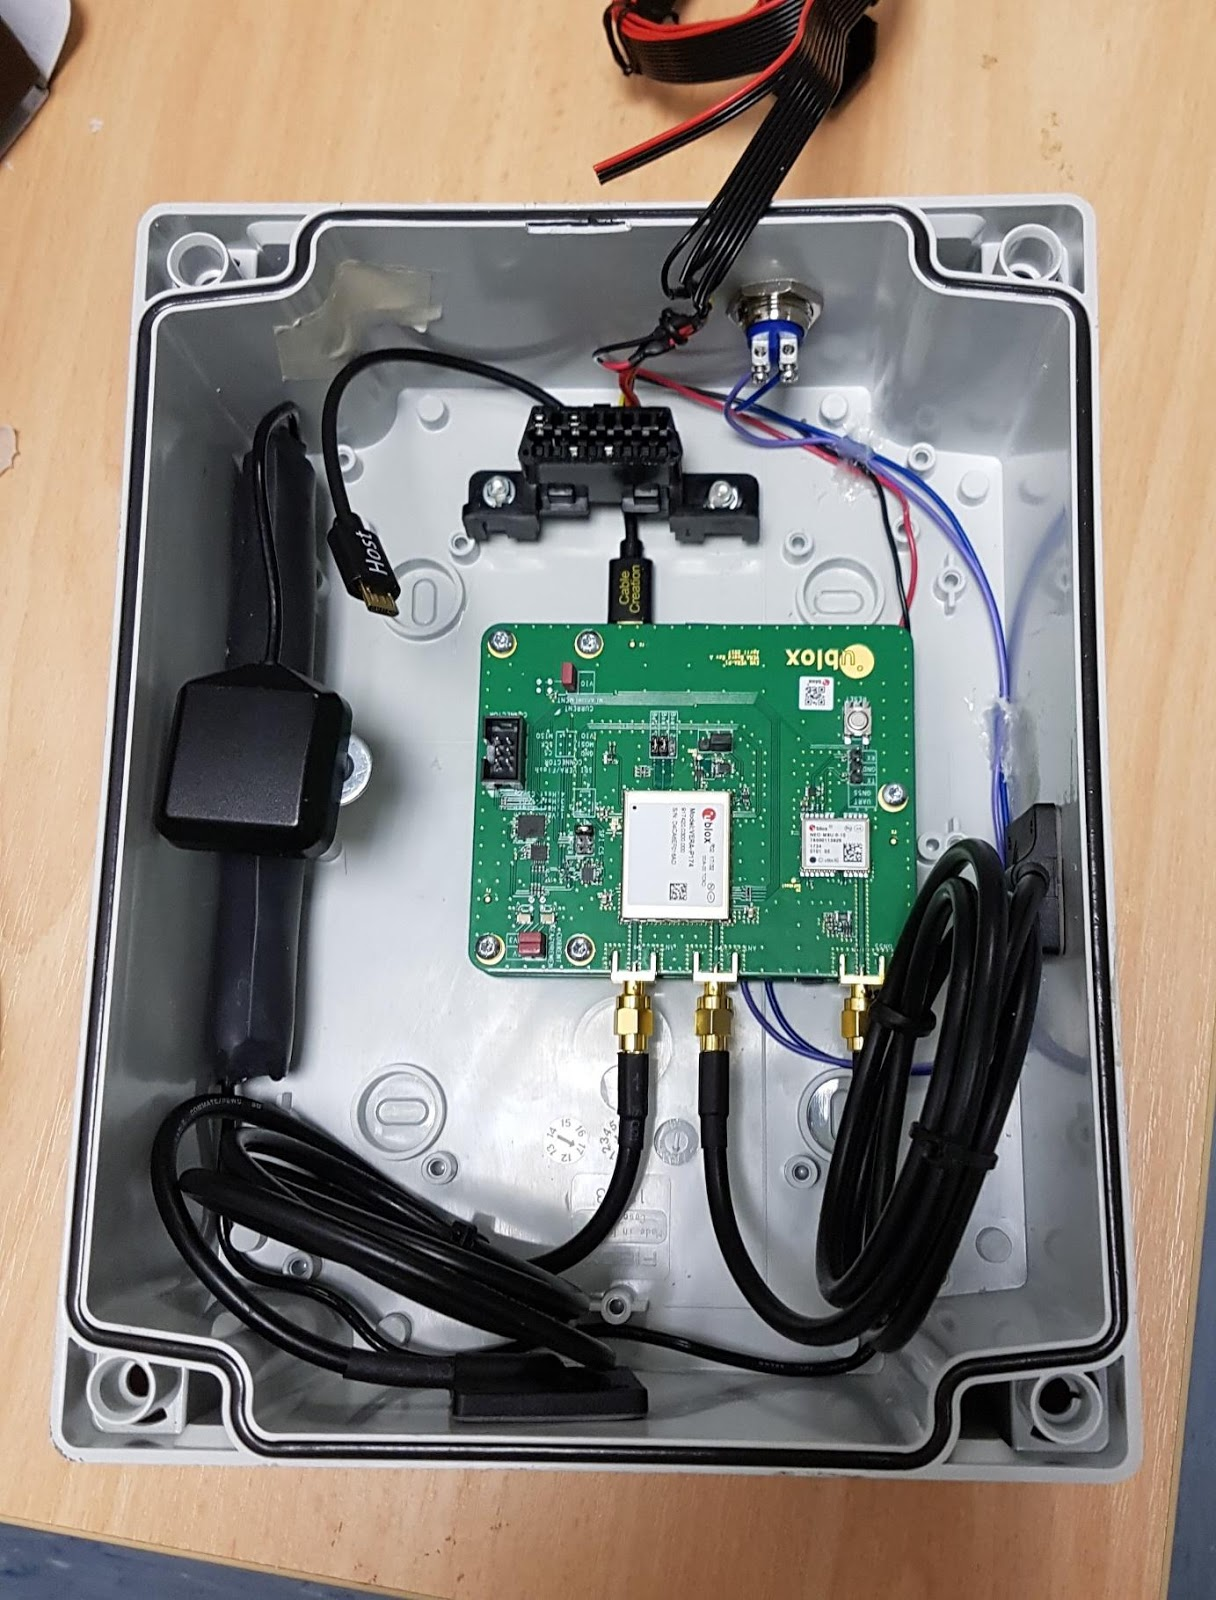
\includegraphics[scale=0.2, angle=90]{\images/v2x_llc.jpg}
                \caption{Prototype llc pour V2X - Vera P174}
            \end{figure}

        \pagebreak

        \subsubsection{Développement effectué}
            Le développement de ce projet est divisé en deux parties:
            \begin{itemize}
                \renewcommand{\labelitemi}{$\bullet$}
                \item Développement des machines à états, un service Morpheus en Java.
                \item Développement de la stack qui remplacerait Marben, en Rust.
            \end{itemize}
            \bigskip
            Les résultats de tests antérieurs avec VolksWagen étaient positifs pour les
            \gls{cam}s. Par contre, la gestion des \gls{denm}s nécessite des machines
            à états ne faisant pas partie de la stack Marben. La stack est, en fait,
            capable d'envoyer et recevoir les \gls{denm}s, mais pas de gérer leur logique.
            J'ai commencé donc le développement du service Morpheus contenant la logique de
            gestion des \gls{denm}s, comme décrit dans la figure \ref{v2x_sm}.

            \begin{figure}[ht]
                \centering
                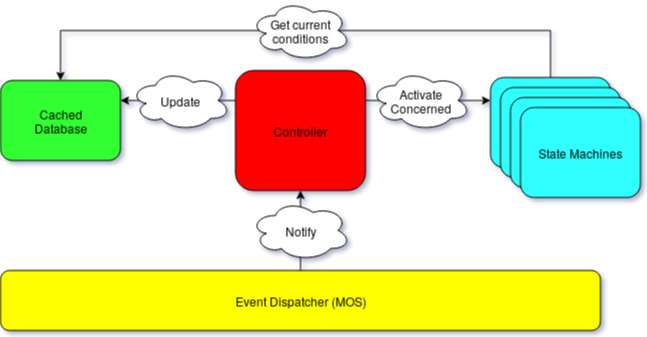
\includegraphics[scale=0.8]{\images/v2x_sm.jpg}
                \caption{V2X State Machines}
                \label{v2x_sm}
            \end{figure}

            Quand un paramètre d'interêt pour une de nos machines change,
            le controlleur est notifié. Il met à jour son cache, et active
            les machines à états concernées. Celles-ci effectuent leurs
            transitions, et déclenchent les actions correspondantes.

    \subsection{Tests \& Performance}
        Un déplacement en Allemagne, à Wolfsburg, nous a vu avancer dans ce projet.
        Malheureusement, il arrive à sa fin prématurée quand VolksWagen nous
        annonce que l'entreprise n'investira pas de ressources dans le projet
        avant une ou deux années. Le projet est alors marqué comme un succès,
        mais arrêté jusqu'à nouvel ordre.
